\section{Auswertung}
\label{sec:Auswertung}
\subsection{Messgrößen und Fehler}
Die Reserviore werden jeweils mit 
\begin{equation}
  V_{\text{Reservior}} = 4 Liter
  \label{eqn:v}
\end{equation}
Wasser befüllt. Desweiteren werden die Temperatur T1 und T2, der Druck $p_{\text{b}}$ und $p_{\text{a}}$ sowie die Leistung des Kompressors jede Minute von dem Messinstrumenten abgelesen. Die Messdaten werden in Tabelle \ref{tab:Daten} aufgelistet. Die Wärmekapazität der Reservoire beträgt 
\begin{equation}
  C_{\text{Reservoire}} = 750 \frac{J}{K} 
  \label{eqn:c_re}
\end{equation}

\begin{table}
  \centering
  \begin{tabular}{c c c c c c}
    \toprule
    $t$ / s & $T_{\text{1}}$ / K & $p_{\text{b}}$ / kPa & $T_{2}$ / K & $P_{\text{a}}$ / kbar & Leistung / kW \\
    \midrule
    0 	& 294.1 & 466	& 294.3	& 496	& 0	\\
    1 	& 294.7 & 608	& 294.3	& 425	& 1.18	\\
    2 	& 295.9 & 618	& 293.2	& 446	& 1.2	\\
    3 	& 296.9 & 638	& 292.5	& 466	& 1.25	\\
    4	& 298.2	& 628	& 291.3	& 466	& 1.25	\\
    5	& 299.4 & 709	& 290.2	& 466	& 1.25	\\
    6	& 300.7 & 730	& 289.3	& 466	& 1.25	\\
    7	& 302.0 & 760	& 288.5	& 455	& 1.25	\\
    8	& 303.2	& 790	& 287.7	& 445	& 1.25	\\
    9	& 304.4 & 812	& 287.0	& 425	& 1.24	\\
    10	& 305.5 & 820	& 286.3	& 425	& 1.24	\\
    11 	& 306.6 & 840	& 285.6	& 415	& 1.23	\\
    12	& 307.6	& 861	& 284.9	& 405	& 1.23	\\	
    13	& 308.7 & 891	& 284.1	& 405	& 1.23	\\	
    14 	& 309.7 & 911	& 283.5	& 395	& 1.23	\\
    15 	& 310.7 & 922	& 282.8	& 395	& 1.24	\\
    16 	& 311.6	& 963	& 282.2	& 385	& 1.25	\\
    17	& 312.5	& 993	& 281.5	& 385	& 1.25	\\
    18	& 313.5	& 1003	& 281.0	& 375	& 1.25	\\
    19	& 314.3	& 1023	& 280.5	& 365	& 1.25	\\
    20	& 315.2	& 1044	& 280.0	& 365	& 1.25	\\
    21	& 316.0	& 1064	& 279.5	& 365	& 1.25	\\
    22	& 316.8	& 1094	& 279.0	& 365	& 1.25	\\
    23	& 317.5	& 1104	& 278.6	& 355	& 1.25	\\
    24	& 318.3	& 1115	& 278.3	& 355	& 1.25	\\
    25	& 319.0	& 1135	& 277.9	& 355	& 1.25	\\
    26	& 319.8	& 1155	& 277.5	& 345	& 1.25	\\
    27	& 320.5	& 1175	& 277.2	& 345	& 1.25	\\
    28	& 321.2	& 1196	& 276.9	& 345	& 1.25	\\
    29	& 321.8	& 1216	& 276.6	& 345	& 1.25	\\
    30	& 322.5	& 1226	& 276.3	& 345	& 1.25	\\
    31	& 323.3	& 1236	& 276.1	& 354	& 1.25	\\
  \end{tabular}
  \caption{Dem Versuchsaufbau entommene Messgrößen}
  \label{tab:Daten}
\end{table}

Zu beachten ist das alle Messgrößen einen Messunsicherheit besitzen, einerseits eine Ablesefehler bei analogen Messinstrumenten als auch einen Technischen.
\begin{eqnarray*}
  \Delta p =& &\pm 10 \text{kp}				\\
  \Delta C =& &\pm 10 \frac{\text{J}}{\text{K}}		\\
  \Delta V =& &\pm 1.6 \text{mL}				\\
  \Delta \rho =& &\pm 13 \frac{\text{kg}}{\text{m$^2$}}	\\
\end{eqnarray*}
Die Messunsicherheit der Dichte für Wasser kommt daraus zu stande, dass Wasser bei verschiedenen Temperatruren seine Dichte ändert.
\begin{figure}
  \centering
  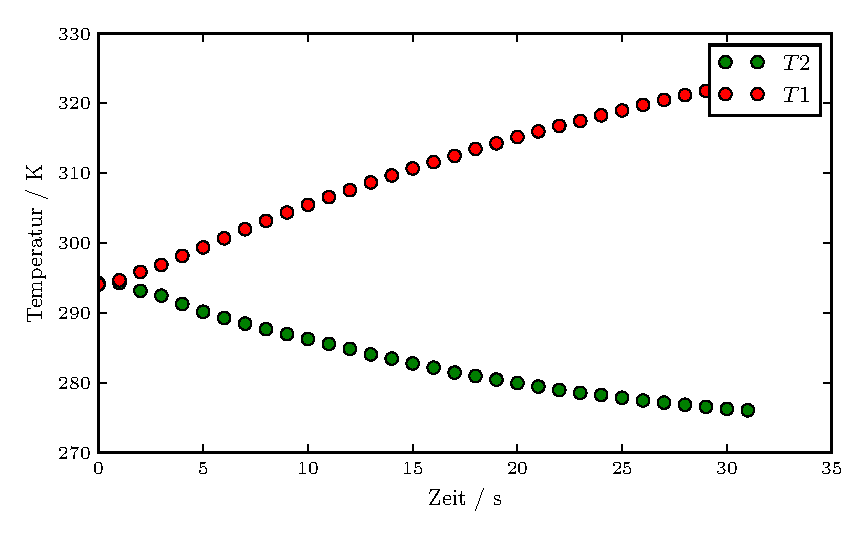
\includegraphics[width=\textwidth]{TVerlauf.pdf}
  \caption{Temperaturverläufe T1 und T2}
  \label{fig:T1&T2}
\end{figure}
\subsection{Näherungsfunktion}
Mit einer nicht-linearen Ausgleichsgraden soll der Temperaturverlauf mit Hilfe der Gleichung approximiert werden. Eine Approximation soll mittels eines Polynoms 2-Grades erfolgen.
\begin{equation}
  T(t) = At^2 + Bt +C
  \label{eqn:ausgleichsgrade}
\end{equation}
Die Ermittelung der Ausgleichsgraden erfolgtmit hilfe von Python 3.4.3. 
